% Figure from MATH 591 notes, section 72 (Lecture 27). ADDED (not from lecture).
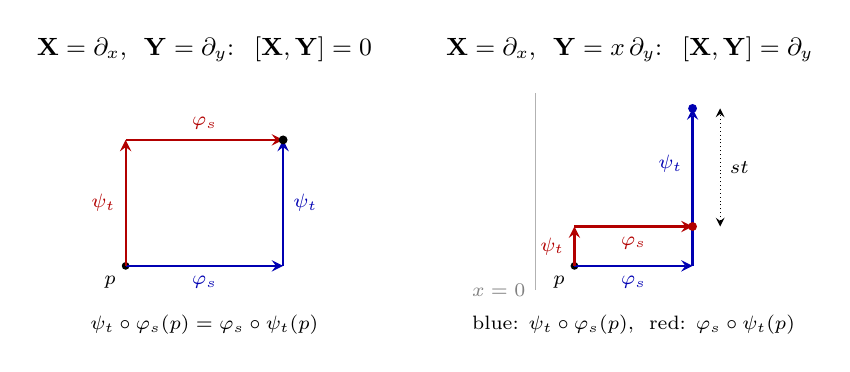
\begin{tikzpicture}[scale=1.0, >=stealth]
\begin{scope}
\node[font=\small] at (1.0,2.75) {$\mathbf{X} = \partial_x$, \ $\mathbf{Y} = \partial_y$: \ $[\mathbf{X}, \mathbf{Y}] = 0$};
\fill (0,0) circle (1.4pt) node[below left, font=\scriptsize] {$p$};
\draw[->, thick, blue!70!black] (0,0) -- node[below, font=\scriptsize] {$\varphi_s$} (2,0);
\draw[->, thick, blue!70!black] (2,0) -- node[right, font=\scriptsize] {$\psi_t$} (2,1.6);
\draw[->, thick, red!70!black] (0,0) -- node[left, font=\scriptsize] {$\psi_t$} (0,1.6);
\draw[->, thick, red!70!black] (0,1.6) -- node[above, font=\scriptsize] {$\varphi_s$} (2,1.6);
\fill (2,1.6) circle (1.6pt);
\node[font=\scriptsize, align=center] at (1.0,-0.75) {$\psi_t \circ \varphi_s(p) = \varphi_s \circ \psi_t(p)$};
\end{scope}
\begin{scope}[xshift=5.2cm]
\node[font=\small] at (1.2,2.75) {$\mathbf{X} = \partial_x$, \ $\mathbf{Y} = x\,\partial_y$: \ $[\mathbf{X}, \mathbf{Y}] = \partial_y$};
\draw[gray!60] (0,-0.3) -- (0,2.2); \node[gray, font=\scriptsize, anchor=north east] at (0,-0.1) {$x = 0$};
\fill (0.5,0) circle (1.4pt) node[below left, font=\scriptsize] {$p$};
\draw[->, thick, blue!70!black] (0.5,0) -- node[below, font=\scriptsize] {$\varphi_s$} (2.0,0);
\draw[->, thick, blue!70!black] (2.0,0) -- node[pos=0.65, left, font=\scriptsize] {$\psi_t$} (2.0,2.0);
\draw[->, thick, red!70!black] (0.5,0) -- node[left, font=\scriptsize] {$\psi_t$} (0.5,0.5);
\draw[->, thick, red!70!black] (0.5,0.5) -- node[below, font=\scriptsize] {$\varphi_s$} (2.0,0.5);
\fill[blue!70!black] (2.0,2.0) circle (1.6pt); \fill[red!70!black] (2.0,0.5) circle (1.6pt);
\draw[<->, densely dotted] (2.35,0.5) -- node[right, font=\scriptsize] {$st$} (2.35,2.0);
\node[font=\scriptsize, align=center] at (1.25,-0.75) {blue: $\psi_t \circ \varphi_s(p)$, \ red: $\varphi_s \circ \psi_t(p)$};
\end{scope}
\end{tikzpicture}
